\chapter{Conceitos Gerais e Revisão da Literatura}
Neste capítulo deve ser proporcionado o estado da arte / referencial teórico
sobre o tema a que se refere o estudo. Um bom pesquisador não deve repetir
trabalhos já concluídos ou que já estão em andamento. Por isso esta sessão é
onde o autor demonstra até onde vai a pesquisa atual no campo de estudos em
questão e estabelece as bases sobre as quais desenvolverá o estudo proposto. A
seguir são mostrados alguns exemplos de como deve-se inserir as figuras e
tabelas. A Figura \ref{fig:exemplo} mostra um exemplo de como inserir uma
figura no texto. A Tabela \ref{tb:exemplo} mostra o exemplo de como uma tabela
deve ser inserida.  Voce pode referenciar capítulos e seções adicionando labels
à elas. Por exemplo, descrevemos a introdução no Capítulo
\ref{chp:introduction}.

\section{Escala de Serviço}
Teste.

\subsection{Eloy}
O programa foi desenvolvido para auxiliar o Sargenteante a escalar os serviços em unidades militares;

Permite montar até 30 escalas que poderão ser definidas pelo próprio operador (Plantão, Gda, Sgt Dia, Of Dia, etc) possibilitando controlar até 500 militares;

O operador pode incluir ou excluir dias na Escala Vermelha ;

As Escalas Vermelhas são montadas ANTES das Pretas (elas são prioritárias) ;

O programa permite que o operador altere as quantidade de postos dos serviços durante a escalação. Isto possibilita: a) a criação de escalas específicas para os dias de meio-expediente (Escala Azul); b) a escalação de serviços cuja responsabilidade da Sub-Unidade ocorra apenas em determinados dias (são aqueles que eventualmente não são escalados TODOS os dias como Cmt Gda e Patrulha); c) que os serviços possam ter número variável de postos ao longo do tempo (0,1,2, etc militares escalados em determinado dia);

Ainda durante os trabalhos de escalação, o operador poderá "forçar" a escalação de um militar em determinado dia e serviço. De forma semelhante, poderá "evitar" que um militar seja escalado em determinado dia e serviço;

A iniciação do Sistema - primeiro uso - é muito facilitada com a guia "Primeira Utilização". Ela orienta o operador na passagem do antigo Sistema (manual) para o novo Sistema (automático).

Com o Módulo de Consultas, o operador poderá obter por exemplo: a quantidade de serviços de cada um dos integrantes das escalas; a relação dos militares que estavam de serviço em determinado dia; a relação de todos os serviços a que determinado militar concorre; a relação dos serviços separadamente nas escalas Vermelha ou Preta; etc);

A realização de Cópias de Segurança é facilmente executada, podendo-se gravar os dados em um "pendrive" para utilização até mesmo em outro computador;

A fotografia e o título existentes na capa do sistema podem ser substituídos pelo nome da Unidade/Subunidade e por uma fotografia livremente escolhida pelo usuário;

O programa possui um Manual "on-line" com as orientações necessárias para que os usuários possam tirar o máximo proveito das facilidades oferecidas pelo Sistema;

O programa procura atender a todas as especificações contidas no RISG ;

Por tratar-se de uma Versão inicial, alguns erros ainda poderão ocorrer, bem como melhorias terão que ser feitas para dar ao Sistema maior funcionalidade. Por essa razão, sugestões e observações serão muito bem-vindas;

O programa roda nas plataformas Windows XP e Vista. Para rodar em Windows 7, 8 e 10 o setup deve ser executando como "administrador" (veja em "Como Instalar");

O desenvolvedor oferece o programa para livre utilização pelas Organizações Militares, estando liberado o download para as mesmas.\citep{eloy}.

\subsection{Planilha Escala Servico Militar Completa}

\begin{table}[htb]
\caption{Características Principais}
\label{tb:exemplo}
\centering
\begin{tabular}{|l|c|r|r|} %left, center, right. Você pode mudar isso
\hline
Desenvolvedor & VASCONEXCEL\\
Nome do software para escritório & Planilha Escala Serviço Militar\\
Modelo & Completo\\
Versão & 1.0 \\
Tempo de licença & 1000 meses \\
Formato	& Digital \\
\hline
\end{tabular}
\end{table}

Planilha de EXCEL criada para auxiliar no controle de efetivo
Controla e gerencia o efetivo de forma simples, intuitiva e objetiva

Funciona somente no EXCEL 2010 em diante (não funciona no LibreOffice)

O arquivo é enviado compactado (.zip) para o email assim que a compra é confirmada.

Especificações da versão COMPLETA:
- Efetivo máximo de 500
- Trabalha com Escalas Internas, Externas, Especiais e Proporcionais
- Cadastra 20 de escalas de cada
- Cadastra 20 destinos diversos
- Cadastra 20 diferentes postos ou graduações
- Gera relatório de previsão das escalas, aditamento, pernoite e mapa da força

Especificações gerais:
- Título principal a critério do usuário
- Imagem da página principal pode ser modificada
- Cor de fundo pode ser alternada em Verde, Azul, Amarelo e Vermelho
- O calendário da escala faz a contagem das escalas em Vermelha, Preta e tem a opção da cor Azul (roxa)

Atenção!
Não é fornecido de maneira alguma a senha para desbloqueio da planilha. Pois se houver modificações da estrutura (simples mudanca de um nome de uma aba ou título de cabeçalhos, excluir ou incluir linhas ou colunas) isso ira interferir diretamente no VBA e comprometer de forma crítica o funcionamento do arquivo.\citep{planilha}

\subsection{Escala de Serviço para Unidades Militares}
Todos os militares estão sujeitos a escalas de serviço e existem várias. Só na casa-mãe de todos os pára-quedistas já estive integrado nas seguintes escalas de serviço, entre outras:

Sentinela à porta de armas e ronda móvel
Cabo auxiliar do comandante da guarda
Sargento de dia à Companhia de Instrução Aeroterrestre
Comandante da Guarda
Largador
Chefe da Área de Embarque
Uma das dificuldades com a nomeação de pessoal para determinada escala, é conseguir escalar o pessoal de forma justa, usando critérios uniformes com uma boa dose de bom senso e ginástica mental. Para ajudar nesta tarefa, desenvolvi uma aplicação para acompanhar o escalador a melhor nomear o pessoal.

A folha de apresentação do programa. É possível configurar uma escala de serviço até 10 militares (para a mesma escala).

\begin{figure}[!htb]
    \centering
    \caption{Tela Ínicial da Planilha}
    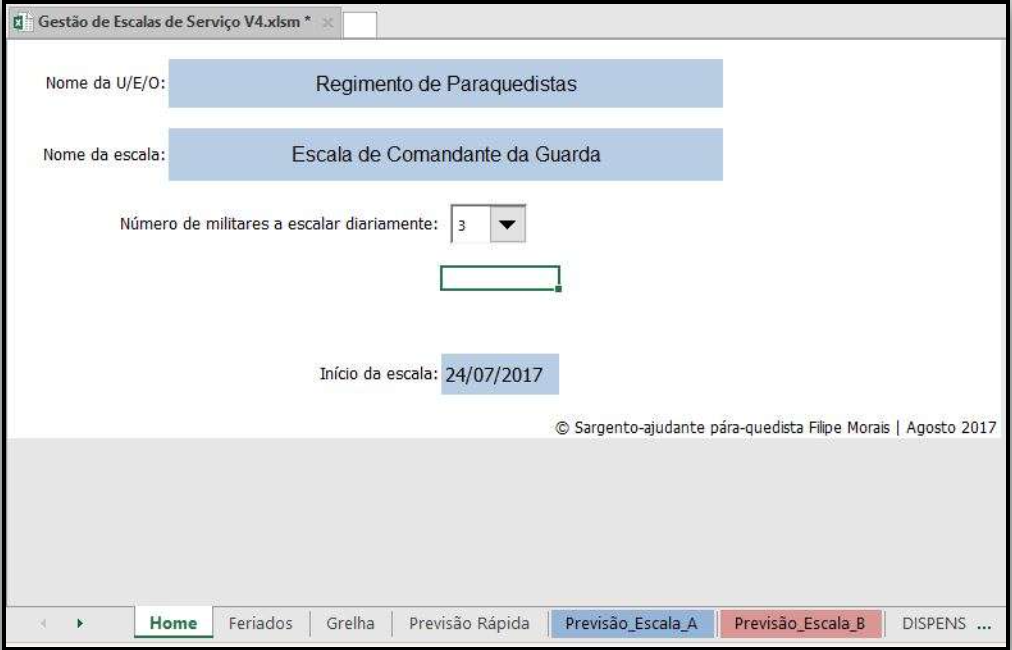
\includegraphics[width=0.35\textwidth]{images/04 - ESUM.png}

    {\footnotesize Fonte: Página oficial do Programa\protect\footnotemark}
    \label{fig:arduino_uno}
\end{figure}

Na grande maioria dos serviços militares existem dois tipos de escala:

A escala A - definida para os dias de semana;

A escala B - definida para os feriados e fins-de-semana.

Assim e por forma a que o programa reconheça os feriados, é necessário introduzi-los no mesmo.

\begin{figure}[!htb]
    \centering
    \caption{Tela de Fériado}
    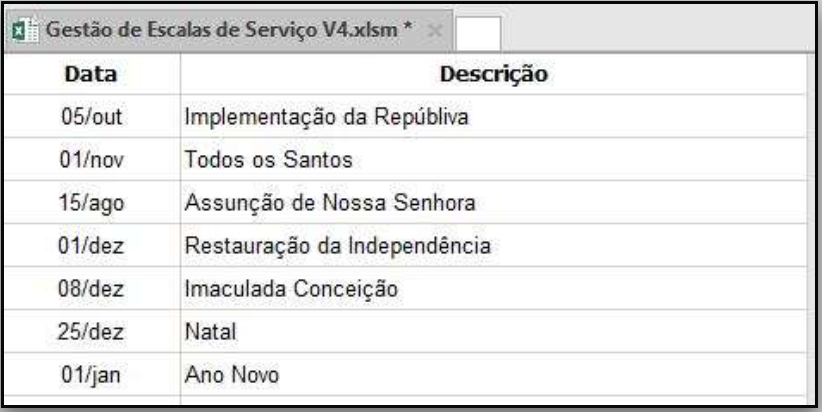
\includegraphics[width=0.35\textwidth]{images/03 - ESUM.png}

    {\footnotesize Fonte: Página oficial do Programa\protect\footnotemark}
    \label{fig:arduino_uno}
\end{figure}

O programa permite obter uma visualização imediata dos próximos a fazer serviço ou seja, uma lista ordenada por ordem dos mais folgados na escala.


\begin{figure}[!htb]
    \centering
    \caption{Tela dos Militeres Escalado}
    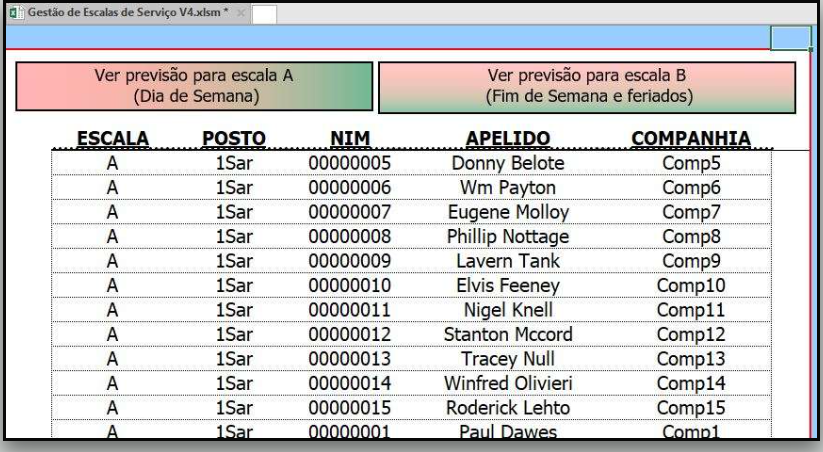
\includegraphics[width=0.35\textwidth]{images/02 - ESUM.png}

    {\footnotesize Fonte: Página oficial do Programa\protect\footnotemark}
    \label{fig:arduino_uno}
\end{figure}


O programa permite imprimir uma previsão da escala. Isto permite aos militares integrados na mesma uma maior coordenação e planeamento da vida pessoal com a profissional.

\begin{figure}[!htb]
    \centering
    \caption{Tela de Impressão}
    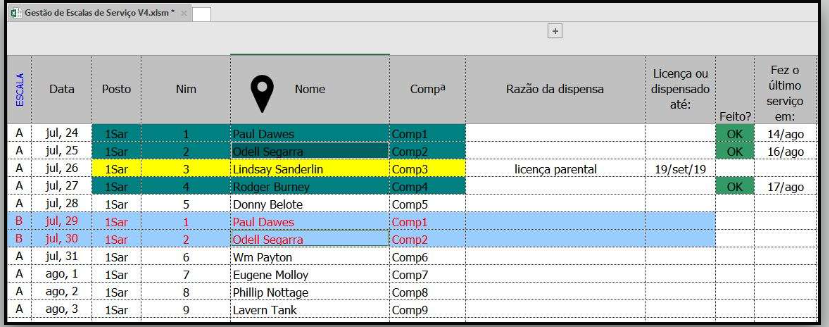
\includegraphics[width=0.35\textwidth]{images/01 - ESUM.png}

    {\footnotesize Fonte: Página oficial do Programa\protect\footnotemark}
    \label{fig:arduino_uno}
\end{figure}

Esta folha é a mais importante do programa. É aqui que vão sendo inseridos os militares conforme vão concluindo o serviço e os próximos a fazer o mesmo.

A forma de o fazer está explicada em detalhe no vídeo, mais abaixo nesta página.

\begin{figure}[!htb]
    \centering
    \caption{Tela dos Militeres Escalado}
    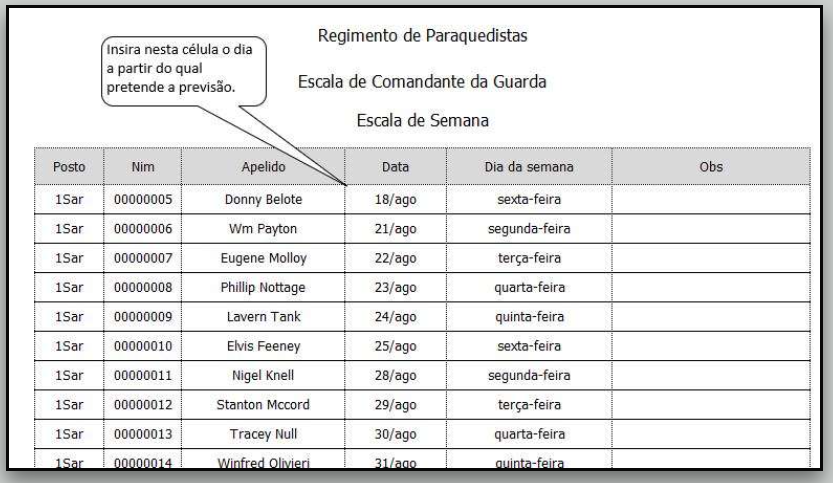
\includegraphics[width=0.35\textwidth]{images/00 - ESUM.png}

    {\footnotesize Fonte: Página oficial do Programa\protect\footnotemark}
    \label{fig:arduino_uno}
\end{figure}

\section{Tecnologias}
Esse capítulo apresenta as tecnologias usadas no desenvolvimento do sistema. Como linguagem de programação, foi utilizado o PHP, acessado via servidor Nginx, com o auxílio do framework Laravel. Para a base de dados, foi utilizado sistema de gerenciador de banco de dados MariaDB. Para orquestrar todos os serviços necessários para subir a aplicação, foi utilizado o Docker.

\subsection{PHP}
Desde sua criação em 1994, a linguagem PHP (Hypertext Preprocessor ou preprocessador de hypertexto, no português), vem sendo amplamente utilizada na web. Mais de 70\% dos sites da web usam PHP no lado do servidor \citep{w3techs}.

A linguagem PHP permite que se trabalhe tanto com servidores windows como servidores linux, a sua evolução permititu que a linguagem abordasse paradigmas estruturados e orientadado a objetos, e comporta diversos bancos de dados, e vem recebendo atualizações constantes, sendo uma lingugem que pode ser tranquilamente utilizada em novos projetos \citep{phpdocs}.
    
\subsection{Laravel}
Laravel é um framework que traz consigo diversas funcionalidades através das suas bibliotecas consolidadas, que vem agregadas ao seu núcleo. Lançado sua primeira versão em 2011, hoje se encontra na versão 9, acompanhando e explorando as novas funcioncionalidades das versões mais atuais do php \citep{laradocs}.
    
O framework hoje conta com 70 mil estrelas no github, o que indica que é um framework bastante conhecido e consolidado no mercado. Atende tanto pequenos quanto grandes projetos, sempre utilizando os padrões mais modernos da linguagem \citep{lararepo}
        
\subsection{Laravel Auditing}
Laravel Auditing, é uma biblitoeca feito para o laravel framework, com o intuito de permitir salvar as mudanças e alterações executadas nas classes de modelo do laravel. Sua configuração padrão permite que registre e recupere os históricos de alterações a partir de uma base de dados, mas também permite que realize a integração com outros meios de logs, como salvar em arquivos ou criar seu próprio driver, para atender a uma necessidade específica \citep{auditdocs}.
    

\subsection{MariaDB}
MariaDB é um sistema gerenciador de banco de dados relacional, que está a mais de 20 anos no mercado.  Sendo um software de codigo aberto, recebe contantes contribuições de comunidades de desenvolvedores que o utilizam, inclusive patches de segurança, tendo esse como um dos principais motivos para utilizá-lo no projeto \citep{mariadbdocs}.
    
\subsection{Nginx}
Escrito por Igor Sysoev, o Nginx é um servidor de proxy reverso HTTP, proxy de servidor de e-mail e um proxy generico de TCP/UDP. Uma de suas características é a possibilidade de configurá-lo em servidores distintos, suportando servidores tanto windows como linux \citep{nginxdocs}.

Oferece um alto desempenho de conexões, sendo seu uso recomendável para aplicações que exigem muitas requisiçoes, ou seja, é escalável e de código aberto.
    
\subsection{Docker}

Docker, tecnologia que divide a aplicação em pequenos containers, tendo cada uma a sua configuração, distinta umas das outras. Permite a entrega rápida de software, e a reprodução do mesmo ambinte tanto pra desenvolvimento quanto homologação e produção \citep{dockerdocs}. 


%\lipsum[2-15]

\let\cleardoublepage\clearpage